\documentclass{hotnets19}

\usepackage{times}  
\usepackage{hyperref}
\usepackage{color, soul}
\usepackage{booktabs}

\hypersetup{pdfstartview=FitH,pdfpagelayout=SinglePage}

\setlength\paperheight {11in}
\setlength\paperwidth {8.5in}
\setlength{\textwidth}{7in}
\setlength{\textheight}{9.25in}
\setlength{\oddsidemargin}{-.25in}
\setlength{\evensidemargin}{-.25in}

\begin{document}

% \conferenceinfo{HotNets 2019} {}
% \CopyrightYear{2019}
% \crdata{X}
% \date{}

%%%%%%%%%%%% THIS IS WHERE WE PUT IN THE TITLE AND AUTHORS %%%%%%%%%%%%

\title{Using Machine Learning to Improve Job Scheduling in Datacenters}

\author{Eli Sherman \and Yash Kumar Lal \and Brian Choi \and Avais Pagarkar}

\maketitle

%%%%%%%%%%%%%  ABSTRACT GOES HERE %%%%%%%%%%%%%%
\begin{abstract}
In modern large-scale computing settings, the order in which jobs are run is critical to the overall performance of the system. Scheduling algorithms, such as Shortest Job First (SJF) and Dominant Resource Fairness (DRF) \cite{ghodsi2011dominant}, are designed to address the issue of determining which jobs to run and when, in order to optimize some criteria. SJF, in particular, is known to be \emph{throughput} optimal \cite{arpaci2015operating}. This algorithm, however, assumes that job runtimes are known when they are scheduled, which is unrealistic except in well-regulated systems. In this paper, we describe efforts to develop an extension to SJF that uses machine learning to predict the runtimes of jobs. To develop and test our algorithm, we implemented a realistic simulation of the Mesos management framework \cite{hindman2011mesos}. We implemented functionality to support running real Flask \cite{Flask}, MapReduce \cite{dean2008mapreduce}, and machine learning training jobs \cite{scikit-learn} and used runtimes of these jobs to train a machine learning regressor to predict future job runtimes. Our results are inconclusive as to whether ML-SJF can improve throughput. As we will explain, this is likely due to the realism of our system implementation.
\end{abstract}

\section{Introduction}

In modern large, parallel systems, such as single-tenant data centers and scientific clusters, there are typically many thousands of active or to-be-run jobs at any given time. Each job has its own requirements for time and space in order to run properly. Due to resource constraints it is not feasible to run all jobs simultaneously and so scheduling algorithms are necessary in order to assign an ordering and allocate resources to the jobs submitted to the system.

Scheduling algorithms are generally designed to optimize one or more criteria such as throughput, fairness, or priority. In modern systems, often the biggest concern in selecting an algorithm is utilization, since even small inefficiencies can cost millions of dollars \cite{Forbes2014}. Algorithms like Distributed Shortest Remaining Time First (D-SRTF) and Shortest Job First (SJF) address this issue by optimizing throughput, where SJF is \emph{provably} throughput-optimal under the assumptions that all jobs arrive simultaneously and that their runtimes can be reliably predicted. Unfortunately, this second assumption only holds under highly constrained systems where jobs are relatively homogeneous.

In light of this, recent work has sought practical methods of predicting the CPU burst time of jobs \cite{slaq, onlinescheduling, dualsimplex}. This has proven to not be a trivial task as the process requires lengthy calculations and a large amount of prior knowledge about the characteristics of a job. In an effort to simplify these calculations and determine defining characteristics of a job that correlates to burst length, others have moved towards machine learning. By gathering a large amount of features from jobs and using their respective run times as the target variable, machine learning models have paved the way for a new domain of possibilities in estimating job runtime length.

A shortcoming of these approaches, however, is that previous attempts to employ machine learning in predicting job runtimes for scheduling have been limited in their generalizability. In particular, these approaches have not collected data from and trained models for use in general datacenter scheduling settings. Instead, they primarily run in production grid settings that do not have the same heterogeneity of jobs inherent in datacenters. Datacenters are uniquely challenging to schedule for due to this heterogeneity and as a result production grid machine learning-based approaches are liable to perform poorly in the datacenter setting (though benchmarking these approaches in a real-world datacenter setting is an open area of research).

In this paper we describe efforts towards developing a machine learning-based SJF scheduling algorithm (ML-SJF), which predicts job runtimes based on the characteristics of jobs submitted to a datacenter framework. In order to achieve a realistic datacenter paradigm, we implemented a simulated version of the Mesos datacenter management framework \cite{hindman2011mesos} with a single master node and a single agent node to run jobs. A heterogeneous set of jobs from three different programming frameworks -- the web framework Flask, MapReduce, and machine learning jobs via sklearn \cite{scikit-learn} -- are submitted to the datacenter and run in a random order. The on-agent runtimes (i.e. the burst times) of these jobs are collected and used for training a hierarchical machine learning model based on support vector regression \cite{chang2011libsvm}, where characteristics of the jobs known at runtime serve as the features.

We compare the performance -- in terms of throughput and average wait time -- of ML-SJF to a randomized SJF, and DRF on a held-out test set of jobs. Our results from cross-validation during training of the ML model show that it is reasonably easy to predict job runtimes. Nevertheless, with respect to system performance, our results are inconclusive as to whether ML-SJF can provide a performance increase over canonical algorithms. Specifically, our implementation performed substantially \emph{worse}, even with accurately predicted runtimes. This is likely due to the nature of our implementation supporting a single agent which poses a problem for resource sharing when larger jobs (i.e. MapReduce jobs) are run simultaneously. This suggests the necessity of further investigation with a more realistic system beyond the scope of this paper.

\section{Scheduling Algorithms}
Several criteria have been proposed for what defines `optimal' scheduling of jobs. All criteria share the goals of reducing resource starvation, either for specific jobs, or for all jobs.
Some of these optimality criteria include:
\begin{itemize}
    \item Maximal Throughput - the total amount of work completed per time unit
    \item Minimal Average Wait Time - the time from when a job is submitted and ready to run until it first begins execution
    \item Minimal Latency - the time from when a job is submitted and ready to run until it is completed (relevant in the case of batch processing)
    \item Maximizing Fairness - ensuring roughly equal resource access, possible conditioned on the priority or workload of each process
\end{itemize}

\subsection{Shortest Job First}

At any given time SJF selects for execution the waiting process with the smallest execution time.
It is a non-preemptive algorithm, meaning that once a job is selected to run, it will run to completion. For this reason, SJF is considered an unfair algorithm as some jobs could be forced to wait a very long time to run as they wait for resources. On the other hand, SJF is provably throughput optimal. That is, the overall throughput of the system will be highest, even though some jobs are starved of resources for a long time.

Because SJF requires accurate estimates of running time for each job (i.e. from an oracle) scheduling in datacenter environments is challenging. Jobs in datacenters are highly heterogeneous with a variety of types (ranging from e.g. low-weight web jobs to heavy-duty MapReduce jobs). Prior work has not adequately addressed the feasibility of obtaining accurate predictions and so SJF could ultimately run jobs in the `wrong' order and not obtain throughput optimality.

\subsection{Dominant Resource Fairness}
In datacenter environments, there are many different types of resources that are required for tasks to run. Previous algorithms targeting fair allocation have primarily focused on a single resource type, such as RAM or storage. DRF \cite{ghodsi2011dominant} is an allocation policy that generalizes the notion of max-min fairness by allowing for multiple resource types. The algorithm tracks the resource utilizations for each user, including a `dominant share' (the resource for which each user has highest utilization). Amongst all jobs submitted to the datacenter, DRF selects the user with the lowest current dominant share and runs one of its jobs (typically selected via FIFO with respect to that user's submitted jobs). The algorithm improves resource sharing among the various users in a datacenter relative to SJF by providing the following fairness oriented properties:
\begin{itemize}
    \item Sharing Efficiency - No user would be better off if resources were partitioned statically and equally among all requesting users
    \item Strategy Proofness - A user cannot a obtain better allocation by lying about the requirements of their jobs
    \item Pareto Efficiency - It does not allocate more resources to a user by taking away resources already allocated to another user
    \item Envy-free - No user prefers the allocation of another user
\end{itemize}

\section{Related Work}
In recent years, there have been several papers that have proposed methods for improving scheduling performance by using statistical analysis on past job runs.

One proposed method to gather approximate job run times is making use of system logs. System logs are reflective of the state of running jobs and resource utilization.
\cite{predictjobcompletion} proposed using hidden markov models to predict job completion times for supercomputing cluster setting.
They first force all log messages to be written in the same template.
Then, since not all log messages are useful for job completion times, sequence mining and frequency distribution analysis are used to select relevant log messages.
Finally, a discrete HMM is trained such that each message has its own transition matrix and emission matrix.
The terminal state in this model is the job residual time, which is predicted every time an important log message is encountered.

\cite{dualsimplex} tackled the task of predicting CPU burst times using a linear programming approach by using the dual simplex method.
This work uses SJF to record waiting, burst and turnaround time of individual processes before converting into a linear programming problem.
An alternate approach for the task is building a fuzzy rule-based system that uses the past history of a process to forecast its next burst time.
However, rule-based systems are limited by the knowledge encoded in them and are not ideal for scalability.

In another attempt to predict CPU burst times for jobs, \cite{helmy2015machine}  tried various ML techniques -- Support Vector Machines (SVM), K-Nearest Neighbor (KNN), Artificial Neural Network (ANN), decision trees -- over a grid workload dataset to learn process runtimes.
This data is composed of various resource requirement features (like number of processors and used memory), timing metrics and job identification attributes (like user ID and group ID).
They apply feature selection techniques to decide which features to use to train their models.
However, such a model does not take into account the heterogeneity of jobs in a datacenter setting.

\cite{onlinescheduling} present an online algorithm to schedule machine learning jobs in distributed clusters.
They decide adjusted numbers of concurrent workers and parameter servers for each long-running job.
Methods also attempt to leverage the iterative aspect of machine learning jobs by collecting quality and resource usage information from concurrent jobs, and then generating highly-tailored quality-improvement predictions for future iterations \cite{slaq}.
Various companies use customized schedulers for to schedule resource-intensive computation jobs.
But such a paradigm is focused on just large-scale machine learning jobs and does not account for heterogeneity.

% To address the variety of possible training objectives in such a scenario, DeepRM \cite{deeprl} present a reinforcement learning agent that tries to incorporate peculiar system features in a generalizable model.

\section{System Design}

In order to make our ML-SJF implementation as realistic and general as possible, we developed a master and agent system that emulates the behavior of the Apache Mesos Management System \cite{hindman2011mesos}. In the interest of limiting the scope for the sake of feasibly completing this course project with a limited time frame, our systems represents a modified version of the full Mesos system. We detail our system design and implementation below. 

\subsection{Master}
In order to ensure a uniform scheduling algorithm and simple interface to work with, we modified Mesos' framework-based scheduling procedure such that the Mesos master directly assigns jobs to worker nodes (the agents). 
Previously the Mesos master scheduled jobs as follows:
\begin{enumerate}
	\item Agents inform the Mesos master of the resources they have to offer
	\item Mesos Master sends resource offers to the frameworks
	\item Frameworks decide which resources to utilize using tasks
	\item Master sends tasks to agents.
\end{enumerate}
Without the framework scheduling abstraction, we no longer need to undergo steps 2 and 3. Instead, our master itself acts as the framework scheduler for the individual jobs, denying jobs that can not be served. Our new master is now in charge of both scheduling jobs and maintaining resource offers, allowing us to maintain a uniform environment to apply our scheduling to.

We now describe the workflow of how the master receives and services job requestions. Figure \ref{fig:master_fsm} gives a finite state machine representation of this workflow.

\begin{figure}[!tbh]
    \centering
    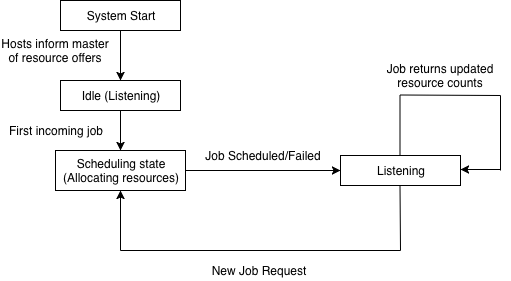
\includegraphics[width=\columnwidth]{hotnets19-template/master.png}
    \caption{Master FSM}
    \label{fig:master_fsm}
\end{figure}

On startup, the master first reads in a list of all jobs from an input text file into a request dictionary and assigns each job to a thread so that jobs can be scheduled and assigned to resources asynchronously. For simplicity of implementation and analysis, jobs are not submitted in real-time and so all jobs `arrive' simultaneously at startup. This design decision was made to accommodate the fact that the frameworks no longer communicate jobs to the master directly. This also allows the master to directly keep track of job runtimes and, by extension, throughput and average job wait time. When assigning jobs to, and receiving completion info from agents, the master uses TCP sockets (described in more detail below). Since each job is assigned it's own thread, the master employs the use of standard synchronization procedures (i.e. semaphores) with respect to modifying shared global variables, such as the request dictionary.

Once the master has received all jobs, it enters a while loop in which it waits for communications from the agents. At first, the communications from the agent will contain resource offers, namely the total resources the agent has. The master keeps track of this information by adding it to a global resources dictionary which it will update as jobs are assigned and completed. Once the master is aware of available resources it can begin sending jobs to that agent.

The other type of communication the master can receive from an agent is a notification that the agent has completed a job request. In this case, the master updates its resource offers, agent resources dictionary, and current utilization of resources (used for DRF) in accordance with the resource release conveyed by the received update. The master also marks the job as completed. Once all jobs have been completed (i.e. a global variable keeping track of jobs left to run is equal to 0), the master can safely exit the while loop. This behavior is correct since the master has a known number of jobs to run at startup.

Upon receiving either type of communication from an agent, if there are still jobs left to run, the master runs a scheduling algorithm using the resource offers and request dictionary to decide which job to run. The master then sends the selected job to an available agent. We implemented three types of scheduling algorithms that the master can use, DRF, SJF and the proposed ML-SJF. Once the master has sent the job to an agent, it decrements the total number of resources that the agent has in the agent resources dict. Once the job is sent, the master will also take the sent job out of the request dictionary. The master repeats this process while also computing and printing the running throughput and average waiting time at each iteration of the while loop.

\subsection{Agent}
Each agent represents a machine capable of executing jobs assigned to it by the user. To ensure that an agent can execute jobs in parallel while also waiting for new jobs, we implemented a multi threaded agent. 

An overview of the flow of the agent can be found in Figure \ref{fig:agent_fsm}.

\begin{figure}[!tbh]
    \centering
    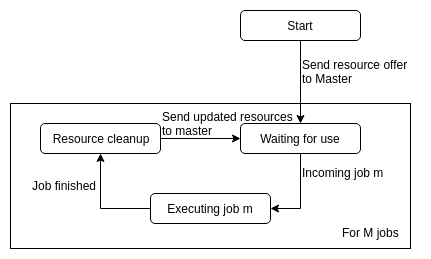
\includegraphics[width=\columnwidth]{hotnets19-template/agent.png}
    \caption{Agent FSM}
    \label{fig:agent_fsm}
\end{figure}

When the agent starts, it is initialized with a list of resources - number of CPUs, number of GPUs, available storage, available memory, alongside a unique Agent ID. After assigning these resources, the agent starts listening on the host machine on port 8000. 

The master connects with the agent by sending a request to the agent on port 8000. As soon as the master claims an agent, the agent gets a list of all its available resources and sends this resource offer to the master. Next, the agent waits for the master to assign it a job. 

Once the agent is assigned a job, it creates a new "child" thread to execute this job as long as the agent has enough resources available to execute the job. The parent goes back to waiting for new jobs. After this, the agent's parent thread repeats this process within a loop. 

The child thread, created by the agent to execute the assigned job, executes the command passed by the master using the subprocess Python module. After the task has finished executing, the child thread then computes the runtime for the job and increases the agent's list of resources to reflect the resources that are now available. Upon completion, the child thread aggregates the runtime and job resources that were previously in use by the process and returns this as an update to the master.
The agent continues accepting jobs and sending updates in a cyclic manner until the master no longer runs. Once the master is done executing, the connection between the agent and master is closed and the agent program exits.

\subsection{Communication}
The master and agent communicate with each other using SocketIO.
Initially, the agent opens a socket to which the master then connects.
As long as this socket is open, both the master and agent can receive communication from each other.
This is crucial since the agent sends an updated resource list after completing any job, which is then used by the master to schedule further jobs.

\section{ML-SJF}
From the standpoint of the Mesos master's scheduling procedure, ML-SJF operates identically to conventional SJF. The difference in the two procedures is that rather being randomly generated, as in our SJF implementation, the predicted runtimes are obtained by performing prediction using our trained model. These predicted runtimes are submitted to the Mesos master at runtime along with the other job information, as in SJF (and DRF, though these predictions are ignored in that algorithm). Below we detail the training data and training procedure.

\subsection{Dataset}
We implemented support for three different types of jobs that can run in our simulated datacenter environment -- web-based, distributed computation and machine learning.
We use Flask \cite{Flask}, MapReduce \cite{dean2008mapreduce} and scikit-learn \cite{scikit-learn} as the frameworks to execute the respective job types. We randomly generated 3000 jobs -- 1000 for each framework -- and their respective features (corresponding to their resource requirements) were randomly chosen by sampling from uniform distributions over the relevant variables (e.g. select an input file uniformly at random; see below).

Each type of job has distinct features associated to it. For MapReduce jobs, we collected several large text files from Project Guttenberg \cite{guttenberg} and created 30 different combinations of these files to serve as inputs. In turn, the features for MapReduce jobs included the size of the job's input files, the number of mappers, and the number of reducers. For sci-kit learn jobs, we used the several of the pre-installed datasets as training data. The features for these jobs included the size of the dataset being used in the job (the number of rows and the number of dimensions), the number of classes the target variable could take on. Finally, for Flask jobs we performed token-sorting with a variety of algorithms and word counting on a large text file, also from Project Guttenberg. The sorting algorithms used were Timsort, Bubble Sort, Insertion Sort, and Bogo Sort. The features for Flask jobs included the file size of the input file and the type of operation -- sorting type or word count. To vary the input sizes, we randomly took subsets of the full file. 

Initially, all the jobs are run and their on-agent runtimes are logged using the conventional SJF algorithm with random predictions for the runtimes.
These runtimes are used for training. We train three separate algorithms, one on each type of job. For predicting job times for our experiments, we use the appropriate trained model for predicting each type of job (i.e. we obtain predictions for Flask job runtimes using the Flask-specific trained model).

\subsection{Support Vector Regression}
Support Vector Regression (SVR) is a flexible modeling approach for performing non-linear regression. For training our models, we used the libsvm implementation of SVR \cite{chang2011libsvm}. We considered both linear and RBF kernels as well as different settings of the regularization parameter in multiples of $10$ from $1$ to $10,000$. We selected the optimal model for each job type via 5-fold cross validation, keeping the model hyper parameters with the best average validation score. In all three cases, cross validation yielded a model with an RBF kernel. This makes intuitive sense since our models are likely to be highly non-linear. For instance, Flask jobs that run Bubble Sort, Insertion Sort, or Bogo sort, will have runtimes that are approximately quadratic (or worse) in the input size.

\section{Results and Evaluation}

To make testing uniform, we packaged the agent in a Docker container and ran the Mesos master and agent from the same node on a Google Cloud Platform virtual machine instance. 
We used an instance with 4 vCPUs and 15GB of RAM.

In order to test all the algorithms, we generated 600 additional jobs not overlapping with the training set. 
We ran these using our Mesos implementation, scheduled by all the algorithms we experiment with.
To compare to ML-SJF, we considered SJF and DRF as baseline algorithms.
For an additional set of experiments with individual framework jobs, we copy the 600 jobs but fix their expected runtimes to be the average runtime of that type of job from the training set.
This is denoted by Hard-coded SJF. 
We report the throughput and average wait time of jobs for these algorithms in Table \ref{all-jobs}. 

\vspace{0.3cm}

\begin{table}[!tbh]
\centering
\begin{tabular}{|c|c|c|}
    \hline
    \textbf{Algorithm} & \textbf{Throughput} & \textbf{Avg Wait Time} \\\hline
    DRF & 0.3522 & 835.95 secs \\\hline
    SJF & 0.4735 & 643.31 secs \\\hline
    ML-SJF & 0.1561 & 1713.26 secs \\\hline
    Hard-coded & 0.1689 & 1734.43 secs \\\hline
\end{tabular}
\caption{Performance of algorithms overall}
\label{all-jobs}
\end{table}

\vspace{0.3cm}

When looking at the throughput for our ML-SJF algorithm compared to the throughputs of the other algorithms, we observe that it has a lower throughput than the conventional SJF and DRF implementations, contrary to our hypothesis.
We suspect that this is because our implementation only has a single agent to which we've assigned jobs to run in parallel.
When we use ML-SJF, because the three types of jobs generally are in three different ranges of runtime, jobs of the same type are executed in order.
In standard SJF, on the other hand, the order of job execution is random.

Executing heavy-weight MapReduce jobs in parallel with other MapReduce jobs is slower than executing them in parallel with either ML or Flask jobs since the two MapReduce jobs are competing for resources and interfering with each other subject to the internal scheduling algorithm of the server's operating system.
For ML-SJF, since MapReduce jobs have the highest predicted runtime, they will only be executed after the lighter-weight jobs (Flask and Scikit-Learn) have finished. The result is a decrease in throughput due to this competition for resources among heavy-weight jobs. This explains the performance of Hard-coded SJF as well. 

Comparing Hard-coded SJF, the predicted runtime of certain jobs submitted by Flask (the quadratic sorting jobs that use insertion sort or bubble sort) were comparable to the runtime of MapReduce jobs. 
As hypothesized above, when Flask jobs are scheduled to run alongside MapReduce jobs, there is less competition for resources (Flask is computationally but not memory intensive). This is a potential explanation for the higher throughput observed in Hard-coded SJF.
To quantify the performance of ML-SJF as compared to SJF for homogenous jobs, we conducted experiments while running only one type of job.
Results from these experiments can be seen in Table \ref{individual-jobs}.

\begin{table}[h]
\begin{tabular}{|c|c|c|c|}
\hline
    \textbf{Job type} & \textbf{Algorithm} & \textbf{Throughput} & \textbf{Avg Wait Time} \\\hline
    MR & SJF & 0.1371 & 310.875 secs \\\hline
    MR & ML-SJF & 0.1375 & 273.97 secs \\\hline
    ML & SJF & 0.1675 & 897.045 secs \\\hline
    ML & ML-SJF & 0.3324 & 437.83 secs \\\hline
    Flask & SJF & 0.1494  & 568.78 secs \\\hline
    Flask & ML-SJF & 0.1393  & 554.29 secs \\\hline
\end{tabular}
\caption{Performance of algorithms with one framework}
\label{individual-jobs}
\end{table}

As we can see from these results, ML-SJF tends to demonstrate higher performance than SJF when there is only one type of job, in terms of both throughput and average waiting time.
This is due to SJF not having the advantage of scheduling different types of jobs together.

\section{Conclusion}
In this paper we describe the implementation of a simulated datacenter which we used to develop a machine learning-based scheduling algorithm, ML-SJF. The datacenter simulation was based on the Mesos Manager with a single master node and, for experiments, a single agent. We gathered empirical data from real framework-derived jobs to train our ML model and then tested the performance of the proposed algorithm relative to well-studied baselines on a test set of jobs in the datacenter simulation.

In the case of homogeneous jobs, we found that ML-SJF performs better than the baselines in terms of both throughput and average waiting time.
However, when considering different types of jobs, ML-SJF schedules similar kinds of jobs simultaneously each other which leads to a degradation of performance on a single agent. As such, the results of this work are inconclusive as to whether or not ML-SJF would be a viable scheduling algorithm.

As future work, the most obvious step would be to generalize the Mesos system to allow for multiple agents. In developing our system, we implemented this functionality but ultimately did not have adequate time to ensure that it could work bug-free due to the added complexity of synchronization and network communication. Beyond this, moving towards a more general ML-SJF could be achieved by training on a much larger, more heterogeneous set of jobs, including the integration of more frameworks. Moreover, a more robust analysis would include testing different proportions of each job type for the input datasets (both test and train) as a generalization of the equal-weight and all-of-one experiments that we ran. Finally, while in testing our system we were able to ensure communication between different physical computers as in a real system, for the sake of a uniform testing environment we used Google Cloud. It would therefore be valuable to benchmark the performance of these methods on a variety of hardware.

\bibliographystyle{abbrv}
\bibliography{hotnets19}

\end{document}

